%\pdfminorversion=4
\documentclass{beamer}
%\documentclass[notes]{beamer}       % print frame + notes
%\documentclass[notes=only]{beamer}   % only notes

%\setbeameroption{show notes on second screen=right}\nofiles{}

\iffalse
	\usepackage{pgfpages}
	\setbeameroption{show notes}
	\setbeameroption{show notes on second screen=right}
	% pdfpc slajdovi.pdf --notes=right
\fi

\usepackage[scaled]{beramono}				% sans-serif monospace
%\usepackage{floatrow} 				% centriranje svih slika
\usepackage{float}					% figure [H]
\usepackage{graphicx} 				% includegraphics
	\usepackage{caption}			% subfigure
	\usepackage{subcaption}			% subfigure
	\usepackage[export]{adjustbox} 	% http://ctan.org/pkg/adjustbox
	\graphicspath{ {./ilustracije/} }		% mapa sa slikama
	\let\oldincludegraphics\includegraphics
	\renewcommand{\includegraphics}[2][]{\oldincludegraphics[#1,max width=0.9\linewidth]{#2}}
\usepackage{tikz} 					% dijagrami
  \tikzset{>=latex}
  \usepackage{pgfplots}
	  \pgfplotsset{every axis/.append style={
	  		axis x line=middle,    	% put the x axis in the middle
	  		axis y line=middle,    	% put the y axis in the middle
	  		axis line style={->},  	% arrows on the axis
	  		xlabel={$x$},          	% default put x on x-axis
	  		ylabel={$y$},          	% default put y on y-axis
	  		samples=100,
	  		axis equal,
	  	}} % axis style
	\usetikzlibrary{fit}
	
\usetikzlibrary{automata,arrows,positioning,calc}
\usetikzlibrary{arrows,%
	petri,%
	topaths}%
	
\usepackage[croatian]{babel}		% teorem

\usepackage{amsmath}

\usepackage{commath}  % abs, norm, derivacije (\od[2]{f}{x}, \od[2]{f}{x} \dif x = dx)


\usepackage{bm}

%\newtheorem{definition}{Definicija}[section]
%\newtheorem{theorem}{Teorem}[section]
%\newtheorem{corollary}{Korolar}[theorem]

\DeclareMathOperator{\step}{step}
\DeclareMathOperator{\Heaviside}{H}
\DeclareMathOperator{\Ramp}{R}
\DeclareMathOperator{\softplus}{softplus}
\DeclareMathOperator{\softmax}{softmax}
\DeclareMathOperator{\logistic}{\sigma}

\newcommand{\mat}[1]{\bm{#1}}
%\newcommand{\m}[1]{\bm{#1}}
\let\vec\relax
\newcommand{\vec}[1]{\bm{#1}}
%\newcommand{\v}[1]{\bm{#1}}
\newcommand{\tens}[1]{\bm{\mathsf{#1}}} 	% undergraduate algebra version

\newcommand{\transpose}{\mathsf T} 	% undergraduate algebra version

\newcommand{\pderiv}[2]{\frac{\partial #1}{\partial #2}}
\newcommand{\deriv}[2]{\frac{\partial #1}{\partial #2}}  % TODO

\DeclareMathOperator*{\argmin}{arg\,min} % thin space, limits underneath in displays
\DeclareMathOperator*{\argmax}{arg\,max} % thin space, limits underneath in displays

\DeclareMathOperator{\sgn}{sgn}

\usepackage{stmaryrd}  % llbracket \rrbracket, ...


%\usepackage{tabularx}
\usepackage{multirow}

\usepackage[multiple]{footmisc}		% višestruke fusnote

\usepackage{dirtree}

\usepackage[hidelinks]{hyperref}

\usepackage{xcolor}
\hypersetup{
	colorlinks,
	linkcolor={blue!50!green!50!black},
	citecolor={green!40!black},
	urlcolor={blue!75!green!30!black}
}

\usepackage[]{algorithmic}

\usepackage{color}
\definecolor{bluekeywords}{rgb}{0.13,0.13,1}
\definecolor{greencomments}{rgb}{0,0.5,0}
\definecolor{redstrings}{rgb}{0.9,0,0}
\usepackage{tabularx}
\usepackage{multirow}

\newcommand{\ilustracija}[1]{\input{ilustracije/#1}}

\iftrue
	\usepackage[croatian]{babel}
	\usepackage[utf8x]{inputenc}	
\fi

\mode<presentation>
{
	\usetheme{Boadilla}      % or try Darmstadt, Madrid, Warsaw, ...
	\usecolortheme{orchid} % or try albatross, beaver, crane, ...
	\usefonttheme{structurebold}  % or try default, serif, structurebold, ...
	\setbeamertemplate{navigation symbols}{}
	\setbeamertemplate{caption}[numbered]
}
\setbeamercolor{structure}{fg=blue!75!green!80!black}	

%\setbeamertemplate{itemize items}[default]
%\setbeamertemplate{enumerate items}[default]
\setbeamertemplate{section in toc}[circle]
\setbeamertemplate{subsection in toc}[circle]
\setbeamertemplate{items}[circle]
\setbeamertemplate{blocks}[default]
\setbeamertemplate{footline}
{
	\leavevmode%
	\hbox{%
		\begin{beamercolorbox}[wd=.15\paperwidth,ht=2.25ex,dp=1ex,center]{author in head/foot}%
			%\usebeamerfont{author in head/foot}\insertshortauthor
		\end{beamercolorbox}%
		\begin{beamercolorbox}[wd=.7\paperwidth,ht=2.25ex,dp=1ex,center]{author in head/foot}%
			\usebeamerfont{title in head/foot}\insertshorttitle  %\hspace*{3em}
		\end{beamercolorbox}%
		\begin{beamercolorbox}[wd=.15\paperwidth,ht=2.25ex,dp=1ex,right]{author in head/foot}%
			\insertframenumber{} / \inserttotalframenumber\hspace*{1ex}
		\end{beamercolorbox}
	}%
	\vskip0pt%
}

\AtBeginSection[]
{
	\begin{frame}<beamer>
		\frametitle{Sadržaj}
		\tableofcontents[currentsection]
	\end{frame}
}


\title{Duboka arhitektura za jednoprolaznu lokalizaciju objekata}
\author{Ivan Grubišić \\ \emph{Voditelj:} Siniša Šegvić}
%\author{Voditelj: Siniša Šegvić}
\institute{Fakultet elektrotehnike i računarstva}
\date{}


\begin{document}
	
\begin{frame}
	\titlepage
\end{frame}


\begin{frame}{Sadržaj}
  \tableofcontents
\end{frame}
\note[itemize]{
	\item prvo nešto reći o neuronskim mrežama, onda opisati izvedbu sustava za semantičku segmentaciju i pokazati rezultate
	\item\item 0:10
}


\section{Uvod}
		
\begin{frame}{Uvod}	
	\begin{itemize}
		\item Razumijevanje sadržaja slike je važan skup problema u računalnom vidu.
		\item Česti zadaci:
		\begin{itemize}
			\item klasifikacija
			\item pronalaženje (engl. \emph{detection}, \emph{localization}) objekata
			\item semantička segmentacija
		\end{itemize}
	\end{itemize}
	\begin{itemize}
		\item U posljednje vrijeme postiže se velik napredak koji se temelji na primjeni dubokih konvolucijskih mreža.
	\end{itemize}
\end{frame}
\note[itemize]{
	\item razumijevanje sadržaja slike osnovni problem RV
	\item u to spada klasifikacija slike - pridjeljivanje odgovarajuće kategorije ili razreda
	\item semantička segmentacija - klasifikacija svakog dijela slike ili piksela
	\item u posljednje vrijeme najbolji rezultati postižu se DKNN
	\item\item 0:30 / 0:40
}


\section{Konvolucijske mreže}

\begin{frame}{Konvolucijske mreže}
	\begin{itemize}
		\item Konvolucijske mreže se sastoje od više slojeva sa svojstvima koja su bolje prilagođena problemima u računalnom vidu.
		\item Slojevi su rijetko i lokalno povezani i dijele se parametri (slika \ref{fig:lok_pov}).
	\end{itemize}
	\begin{columns}[c]	
		\begin{column}{.673\textwidth}
			\begin{block}{Konvolucijski sloj}
				Konvolucijski sloj čini skup naučenih filtara od kojih svaki stvara jednu izlaznu matricu. 
				$$
				\matr{H}_{lp}=\varphi\left(
				-\theta_{lp} + \sum_q \matr{w}_{lpq}\ast\matr{H}_{(l-1)q}\right),
				$$
				gdje su $\matr{H}$ mape značajki, $\matr{w}$ konvolucijske jezgre, $\matr{\theta}$ pragovi, $l$ oznaka sloja, a $q$ i $p$ oznake ulazne i izlazne mape značajki.
			\end{block}
		\end{column}
		\begin{column}{.273\textwidth}
			\begin{figure}[ht] \centering
				\scalebox{0.8}{\ilustracija{konv-sloj}}
				\caption{Jednostavni jednodimenzionalni konvolucijski sloj.}
				\label{fig:lok_pov}
			\end{figure}
		\end{column}
	\end{columns}
\end{frame}

\begin{frame}{Konvolucijske mreže: učenje}
	\begin{itemize}
		\item Neuronska mreža se uči minimizacijom funkcije pogreške.
		\item Parametri mreže se prilagođavaju gradijentnim spustom ili nekim algoritmom koji se na njemu temelji.
		\item Gradijent se računa algoritmom propagacije pogreške unatrag (engl. \emph{backpropagation}).
	\end{itemize}
\end{frame}
\note[itemize]{
	\item učenje algoritmima temeljenim na gradijentnom spustu (prva derivacija)
	\item mreža se optimira minimizacijom funkcije pogreške
	\item ovisno o vrsti problema to mogu biti npr. SKP ili UE
	\item\item 0:30 / 6:20
}


\section{Pronalaženje objekata}

\begin{frame}{Pronalaženje objekata}
	\begin{itemize}
		\item Zadatak je prepoznati objekte i pridružiti im oznake razreda i najmanje opisane okvire.
		\item Sustav obično pronađe velik broj okvira od kojih treba izdvojiti najbolje.
	\end{itemize}
	\begin{figure}[ht] \centering
		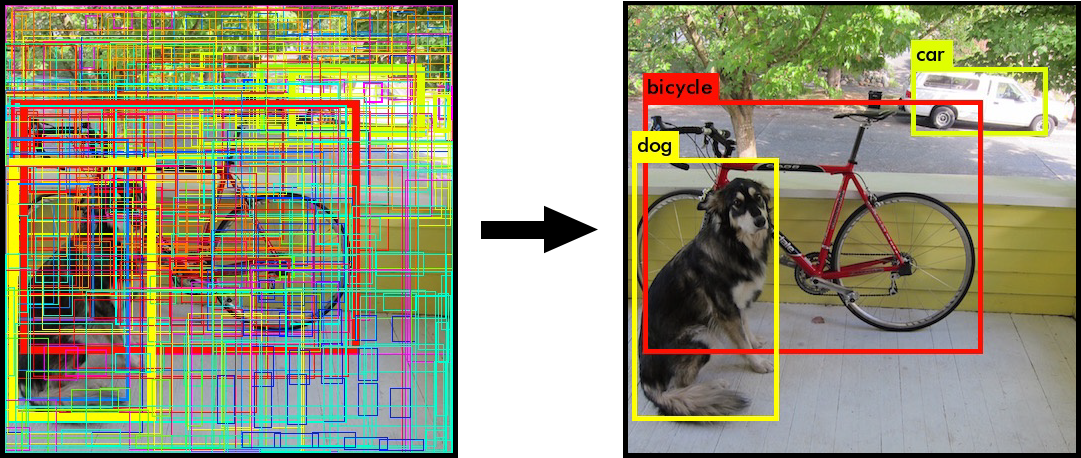
\includegraphics[max width=1\linewidth]{many-boxes}
		\caption{Odbacivanje okvira kandidata i dobivanje konačnih okvira.}
		\label{fig:stanfordbgdsi}
	\end{figure}
\end{frame}


\begin{frame}{Pronalaženje objekata: osnovni pristupi}
	\begin{itemize}
		\item  Najjednostavniji pristup pronalaženju objekata je korištenje pomičnih prozora različitih dimenzija i klasificiranje svake na taj način dobivene podslike.
		\item Do otprilike 2012. godine najuspješniji su bili modeli koji klasificiraju svaki dio slike dobiven pomičnim prozorom i objekte modeliraju dijelovima koji mogu biti različito raspoređeni (engl. \emph{deformable part model}, \emph{DPM}) i kao značajke koriste histogramie gradijenata (engl. \emph{histogram of gradients}, \emph{HoG}).
		\item Malo kasnije su se pokazali uspješnima postupci koji umjesto klasificiranja pomičnog prozora koriste neki način predlaganja okvira  koji služi smanjivanju broja okvira koje treba potpuno klasificirati.
	\end{itemize}
\end{frame}

\begin{frame}{Pronalaženje objekata: evaluacijske mjere}
	\begin{itemize}
		\item  Mjera koja se koristi pri utvrđivanju koji okviri rezultati odgovaraju kojim ciljnim okvirima je omjer površine presjeka i unije ($\mathit{IoU}$, engl. \emph{intersection over union}).
	\end{itemize}
	\begin{block}{Jaccardov koeficijent sličnosti}
		Jaccardov koeficijent sličnosti definiran je kao omjer površine preklapanja i ukupne površine.
		$$
		J(A,B) = \frac{|A\cap B|}{|A\cup B|} = \frac{|A\cap B|}{|A|+|B|-|A\cap B|}.
		$$			
	\end{block}
\end{frame}

\begin{frame}{Pronalaženje objekata: evaluacijske mjere}
	\begin{block}{Preciznost i odziv i mjera $F_1$}
		Preciznost $P$ (engl. \emph{precision}) je udio relevantnih rezultata u svim rezultatima. \\
		Odziv $R$ (engl. \emph{recall}) je udio relevantnih rezultata u svim relevantnim objektima. \\		
		Mjera $F_1$ je harmonijska sredina preciznosti i odziva.
		$$
		P = \frac{\mathit{tp}}{\mathit{tp} + \mathit{fp}}, \quad
		R = \frac{\mathit{tp}}{\mathit{tp} + \mathit{fn}}, \quad
		F_1 = ({P^{-1}+R^{-1}})^{-1}.
		$$			
	\end{block}
	\begin{itemize}
		\item  Okvir rezultat se obično smatra ispravnim ($\mathit{tp}$) ako je njegov koeficijent sličnosti s obzirom na ciljni okvir odgovarajućeg razreda veći od $0.5$ i najveći među koeficijentima sličnosti svih okvira rezultata za koje isto vrijedi.
	\end{itemize}
\end{frame}

\begin{frame}{Pronalaženje objekata: evaluacijske mjere}
	\begin{itemize}
		\item Povećavanjem skupa razmatranih rezultata redom od okvira za čiju je klasifikaciju sustav najsigurniji, preciznost se smanjuje, a povećava se odziv.
	    \only<1> {
	    	\begin{figure}[ht] \centering 
	    		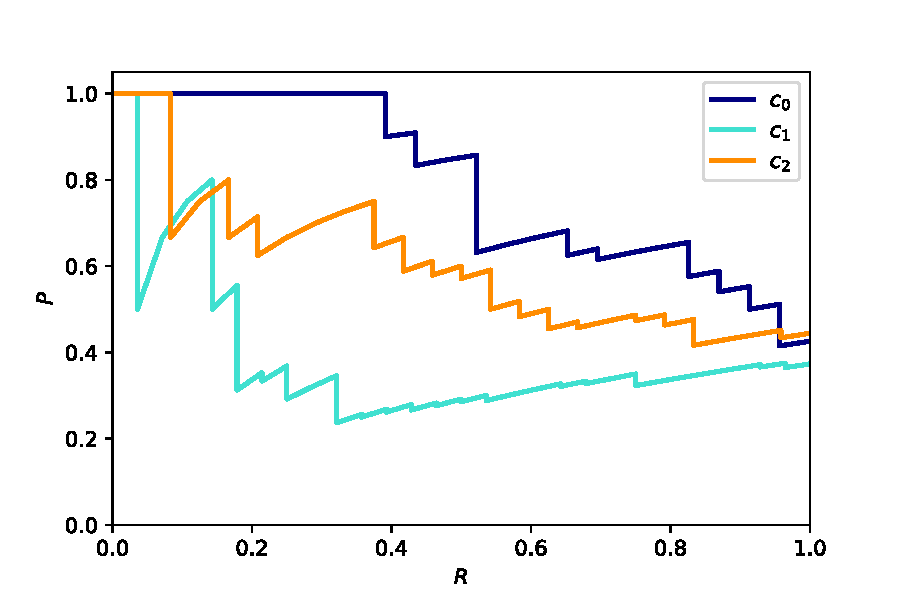
\includegraphics[max width=0.75\linewidth]{pr-curve.pdf}
	    		\caption{Krivulje preciznosti u ovisnosti o odzivu za 3 razreda.}
	    		\label{fig:piramida}
	    	\end{figure}
	    }
	    \only<2> {
			\begin{figure}[ht] \centering 
				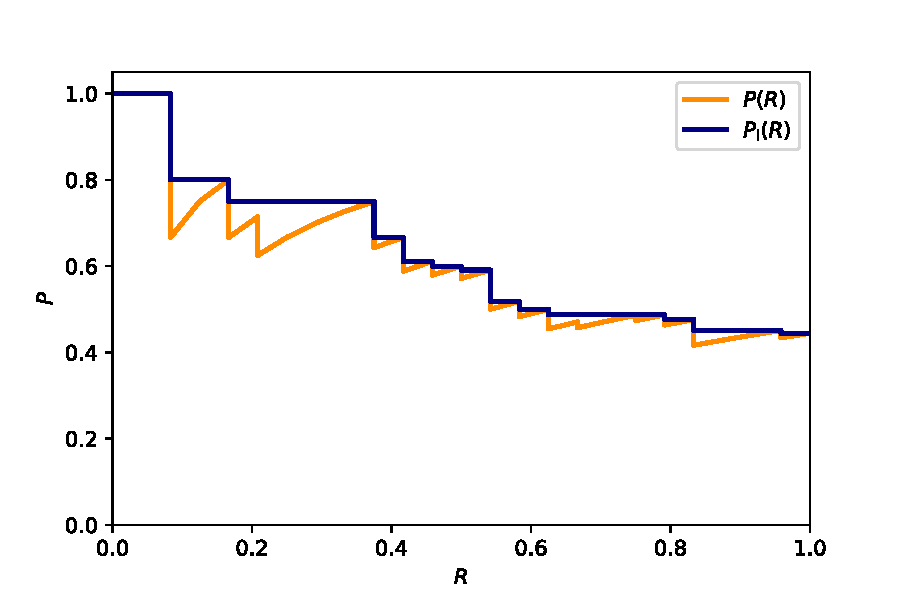
\includegraphics[max width=0.75\linewidth]{pr-interp.pdf}				
				\caption{Krivulja interpolirane preciznosti u ovisnosti o odzivu.}
				\label{fig:piramida}
			\end{figure}
        }			
	\end{itemize}
\end{frame}

\begin{frame}{Pronalaženje objekata: evaluacijske mjere}
	\begin{block}{Srednja preciznost}
		Kao evaluacijska mjera za pronalaženja objekata s jednim razredom se često koristi prosječna (interpolirana) preciznost ($\mathit{AP}$) koja je jednaka površini ispod krivulje preciznosti i odziva:
		$$
		\mathit{AP} = \int_{0}^{1} P(r) \dif r . 
		$$
	\end{block}
	\begin{block}{Srednja prosječna preciznost}	 
		U slučaju više razreda koristi se srednja prosječna (interpolirana) preciznost:
		$$
		\mathit{mAP} = \frac{1}{\abs C}\sum_{c \in C} \mathit{AP}_c .
		$$
	\end{block}
\end{frame}


\section{SSD: Single Shot MultiBox Detector}

\begin{frame}{SSD: Single Shot MultiBox Detector}
	\begin{itemize}
		\item SSD je model za pronalaženje objekata koji se temelji na dubokoj konvolucijskoj mreži.
		\item SSD u jednoj propagaciji unaprijed generira sve predikcije okvira.
	\end{itemize}
	\begin{figure}[ht] \centering 
		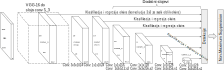
\includegraphics[max width=1\linewidth]{ssd-dijagram}
		\caption{Ilustracija sustava s prikazanim slojevima značajki koje koriste slojevi za klasifikaciju i regresiju okvira.}
		\label{fig:arhitektura}
	\end{figure}
\end{frame}

\begin{frame}{SSD: Single Shot MultiBox Detector}
	\begin{itemize}
		\item Na nekim slojevima značajki konvolucijski se vrši klasifikacija i regresija (prilagodba) dimenzija i položaja razmatranih okvira različitih oblika koji su dodijeljeni svakom položaju u sloju značajki.
	\end{itemize}
	\begin{figure}[ht] \centering
		\begin{subfigure}[b]{0.32\textwidth} \centering
			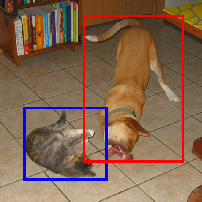
\includegraphics[width=\textwidth]{ssd-truth.pdf}
			\caption{Slika sa željenim okvirima}
		\end{subfigure}
		\begin{subfigure}[b]{0.32\textwidth} \centering
			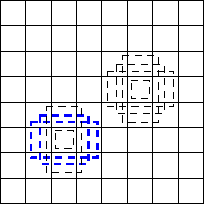
\includegraphics[width=\textwidth]{ssd-8x8fm.pdf}
			\caption{Mapa značajki dimenzija $8\times8$}
		\end{subfigure}
		\begin{subfigure}[b]{0.32\textwidth} \centering
			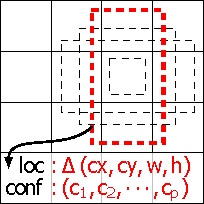
\includegraphics[width=\textwidth]{ssd-4x4fm.pdf}
			\caption{Mapa značajki dimenzija $4\times4$}
		\end{subfigure}
		%TODO: napraviti novu sliku
		\caption{Svakom pikselu nekih slojeva značajki pridruženo je nekoliko razmatranih okvira različitih omjera stranica. Crtkani okviri najbolje odgovaraju ciljnim okvirima i zato su najpogodniji za učenje parametara.}
	\end{figure}
\end{frame}

\begin{frame}{SSD: učenje}
	\begin{itemize}
		\item Za svaku sliku s ciljnim okvirima se iz skupa za učenje prvo među razmatranim okvirima odaberu oni koji su najprikladniji za učenje pozitivnih i negativnih primjera rezultata, a onda se parametri korišteni za dobivanje odabranih okvira prilagođavaju algoritmom koji se temelji na gradijentnom spustu.
		\item $S$ će označavati skup razmatranih okvira, $T$ skup ciljnih okvira, a $C$ skup razreda koji uključuje i razred \emph{ostalo}.
	\end{itemize}
\end{frame}

\begin{frame}{SSD: učenje}
	\begin{block}{Odabir okvira za učenje pozitivnih primjera}
		Za učenje pozitivnih primjera svakom ciljnom okviru se pridružuje podskup razmatranih okvira $S_+ \subseteq S$ u kojemu za svaki element vrijedi:
		\begin{itemize}
			\item koeficijent sličnosti $J$ s nekim ciljnim okvirom je veći od $0.5$ ili
			\item najbolje se od svih preklapa s nekim ciljnim okvirom.		
		\end{itemize}
		$a\colon T\to 2^S$ predstavlja pridruživanje razmatranih okvira ciljnom okviru:
		$$
		a(t) = \{\arg\!\max_s \{ J(t,s) \mid s\in S\}\} \cup \{s\in S\mid J(t,s) > 0.5 \}.
		$$
	\end{block}
	\begin{block}{Odabir negativnih primjera}
		Umjesto korištenja svih negativnih primjera, za učenje se odabire samo njihov podskup koji daje najveći gubitak  klasifikacije i nema više elemenata od $3\left|S_+\right|$. Na taj način se ostvaruje brža i stabilnija konvergencija.
	\end{block}
\end{frame}

\begin{frame}{SSD: učenje}
	\begin{itemize}
		\item Neki okvir $u=(\vect{x}_u, \vect{d}_u, \vect{c}_u)$ određen je vektorima položaja $\vect{x}_u$, dimenzijama $\vect{d}_u$ i pouzdanostima klasifikacije $\vect{c}_u$ dimenzije $\left|C\right|$ koje su u slučaju ciljnog okvira \emph{one-hot}-vektor.
		\item Slojevi za klasifikaciju i regresiju okvira pomake i dimenzije okvira računaju u relativnim koordinatama u odnosu na razmatrane okvire. 
		\item Funkcija $r_s(u)$ preslikava položaj i dimenzije okvira $u$ iz koordinata slike u relativne koordinate razmatranog okvira $s$: 
		$$
			r_s(u) = ((\vect{x}_u-\vect{x}_{s})\oslash\vect{d_s}, \ln\left(\vect{d}_u\oslash\vect{d}_s\right), \vect{c}_u).
		$$
	\end{itemize}
\end{frame}

\begin{frame}{SSD: učenje}
	\begin{block}{Gubitak}
		Gubitak $L$ je definiran kao težinski zbroj gubitka položaja $L_l$ i gubitka klasifikacije $L_c$:
		\begin{align*}
		L &= \frac{1}{\left| S_+\right|}(L_\text{l} + \alpha L_\text{c}), \\
		L_\mathrm{l} &= \sum_{t \in T} \sum_{s \in a(t)} \left(
		\lVert \vect{x}_{\hat{h}_s} - \vect{x}_{r_s(t)}
		\rVert_{\tilde{1}}
		+ \lVert \vect{d}_{\hat{h}_s} - \vect{d}_{r_s(t)}
		\rVert_{\tilde{1}} \right), \\
		L_\text{c} &= -\sum_{t \in T}\sum_{s\in a(t)}\ln c_{s(\arg\max\vect{c}_t)} 
		-\sum_{s\in S_-}\ln c_{s0}.
		\end{align*}
	\end{block}
\end{frame}


\section{Rezultati}

\begin{frame}{Rezultati}
\begin{table}[htbp]
	\centering	
	\resizebox{0.8\textwidth}{!}{%		
	\begin{tabular}{|c|c|c|c|c|}
		\hline
		\multirow{2}{*}{Model} & \multirow{2}{*}{\emph{FPS}} & \multirow{2}{*}{Podaci za učenje} & \multicolumn{2}{c|}{$\textit{mAP}/\%$} \\ \cline{4-5}
		& & & VOC2007 & VOC2012 \\
		\hline
		\multirow{2}{*}{Fast-RCNN} 
		& \multirow{2}{*}{0.5}
		& \footnotesize{VOC07} & 66.9 & - \\ \cline{3-5}
		& & \footnotesize{VOC07, VOC12} & 70.0 & 68.4 \\ \hline
		\multirow{3}{*}{Faster-RCNN}
		& \multirow{3}{*}{7}
		& \footnotesize{VOC07} & 69.9 & - \\ \cline{3-5}
		& & \footnotesize{VOC07, VOC12} & 73.2 & 70.4 \\ \cline{3-5}
		& & \footnotesize{VOC07, VOC12, COCO} & 78.8 & 75.9 \\ \hline
		YOLO & 45 & \footnotesize{VOC07, VOC12} & 63.4 & 57.9 \\ \hline
		*YOLOv2-544 & 40 &  \footnotesize{VOC07, VOC12} & 78.6 & 73.4 \\ \hline
		*PVANET-c & 31 &  \footnotesize{VOC07, VOC12, COCO} & 84.4 & 83.7 \\ \hline
		*PVANET & 22 &  \footnotesize{VOC07, VOC12, COCO} & 84.9 & 84.2 \\ \hline
		\multirow{3}{*}{SSD300}
		& \multirow{3}{*}{46}
		& \footnotesize{VOC07} & 68.0 & - \\ \cline{3-5}
		& & \footnotesize{VOC07, VOC12} & 74.3 & 72.1 \\ \cline{3-5}
		& & \footnotesize{VOC07, VOC12, COCO} & 79.6 & 77.5 \\ \hline
		\multirow{3}{*}{SSD512} 
		& \multirow{3}{*}{19} 
		& \footnotesize{VOC07} & 71.6 & - \\ \cline{3-5}
		& & \footnotesize{VOC07, VOC12} & 76.8 & 74.9 \\ \cline{3-5}
		& & \footnotesize{VOC07, VOC12, COCO} & 81.6 & 80.0 \\ \hline
	\end{tabular}
	}
	\caption{Usporedba rezultata evaluacije na skupovima \emph{VOC2007-test} i \emph{VOC2012-test}}
	\label{tab:rezultati-usporedba-map}
	\end{table}
\end{frame}


\begin{frame}{Rezultati}
\begin{table}
	\centering
	\resizebox{0.8\textwidth}{!}{%		
	\begin{tabular}{|r|cccccc|}
		\hline
		više slojeva značajki za traženje objekata & & $\bullet$ & $\bullet$ & $\bullet$ & $\bullet$ & $\bullet$ \\
		više proširivanja podataka & $\bullet$ & & $\bullet$ & $\bullet$ & $\bullet$ & $\bullet$ \\
		korištenje omjera $\left\{\frac{1}{2},2\right\}$ & $\bullet$ & $\bullet$ & & $\bullet$ & $\bullet$ & $\bullet$ \\
		korištenje omjera $\left\{\frac{1}{3},3\right\}$ & $\bullet$ & $\bullet$ & & & $\bullet$ & $\bullet$ \\
		jezgra $3\times 3$ s dilatacijom 6 u sloju \texttt{fc6} & $\bullet$ & $\bullet$ & $\bullet$ & $\bullet$ & & $\bullet$ \\
		\hline
		$\textit{mAP}/\%$ & 62.4 & 65.5 & 71.6 & 73.7 & 74.2 & \textbf{74.3} \\
		\hline
	\end{tabular}
	}
	\caption{Utjecaj različitih odabira komponenata na srednju prosječnu pogrešku kod modela SSD300 na skupu \emph{VOC2007-test}. Redak "više slojeva značajki za traženje objekata" označava korištenje slojeva značajki \texttt{conv4\_3}, \texttt{conv7}, \texttt{conv8\_2}, \texttt{conv9\_2}, \texttt{conv10\_2} i \texttt{conv11\_2} umjesto samo \texttt{conv7} za pronalaženje objekata.}
	\label{tab:kanaliza-komponenata}
\end{table}
\end{frame}

\begin{frame}{Rezultati}
	\begin{figure}
		\centering
		%\resizebox{0.8\textwidth}{!}{%		
		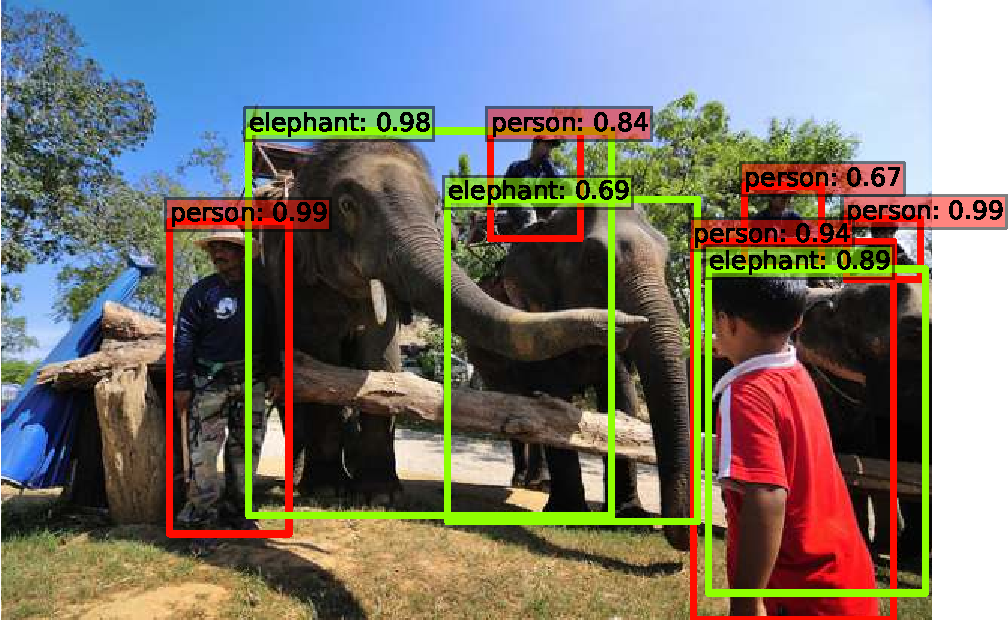
\includegraphics[trim={0 0 0 0.6cm},clip,width=0.22\linewidth]{ilustracije/coco/388513}
		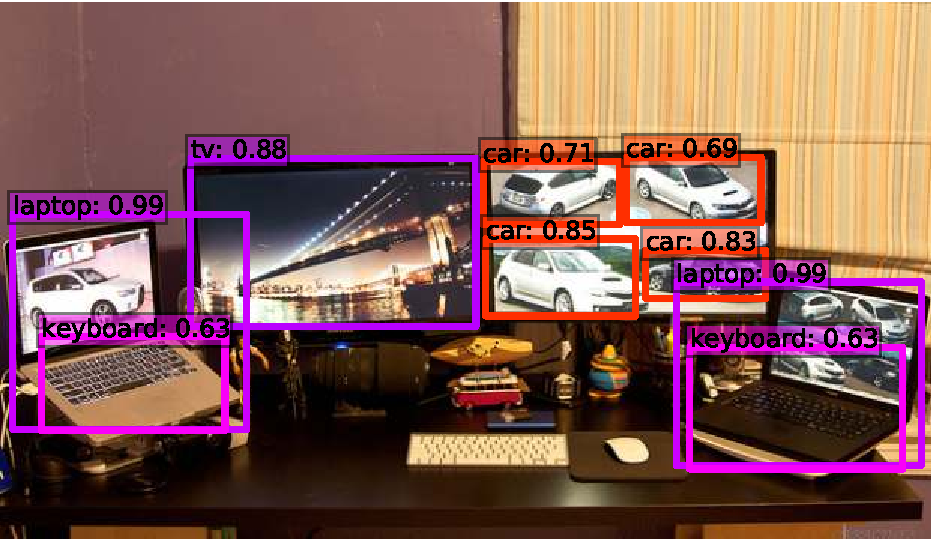
\includegraphics[width=0.22\linewidth]{ilustracije/coco/420454}
		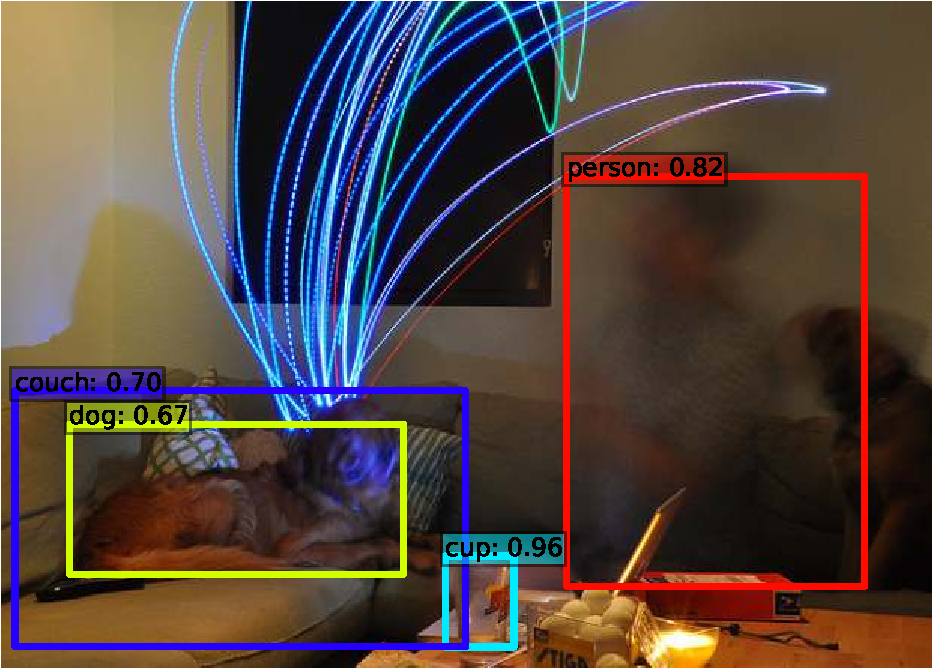
\includegraphics[trim={0 0 0 2.2cm},clip,width=0.22\linewidth]{ilustracije/coco/230476}
		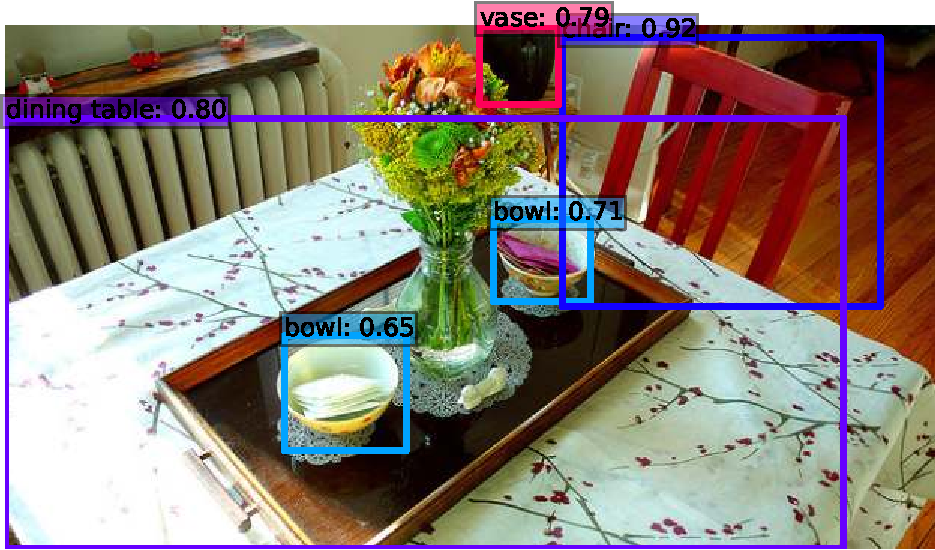
\includegraphics[width=0.22\linewidth]{ilustracije/coco/96709}\\
		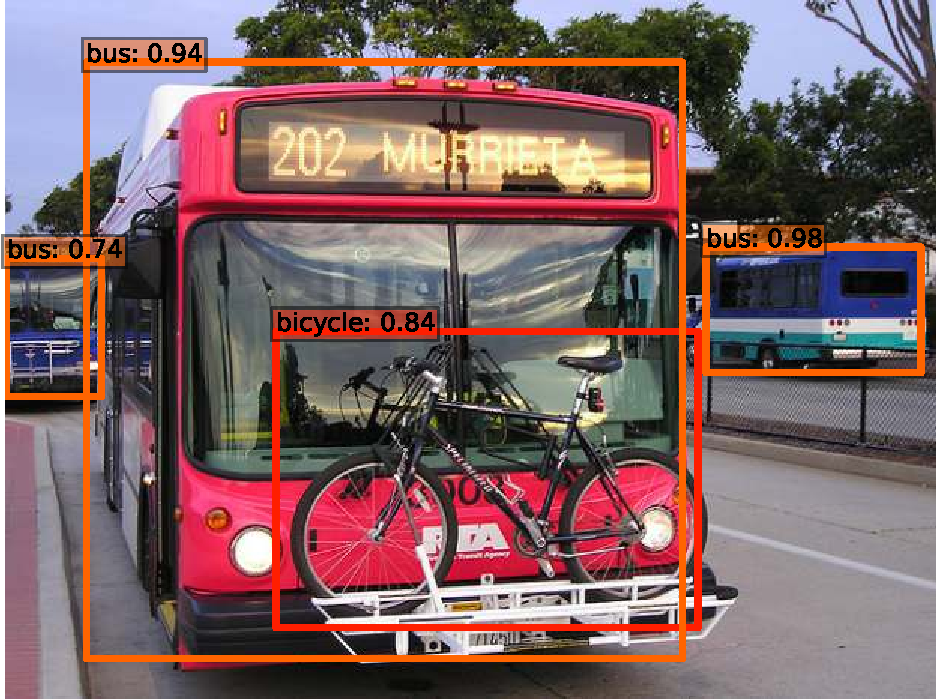
\includegraphics[width=0.22\linewidth]{ilustracije/coco/440980}
		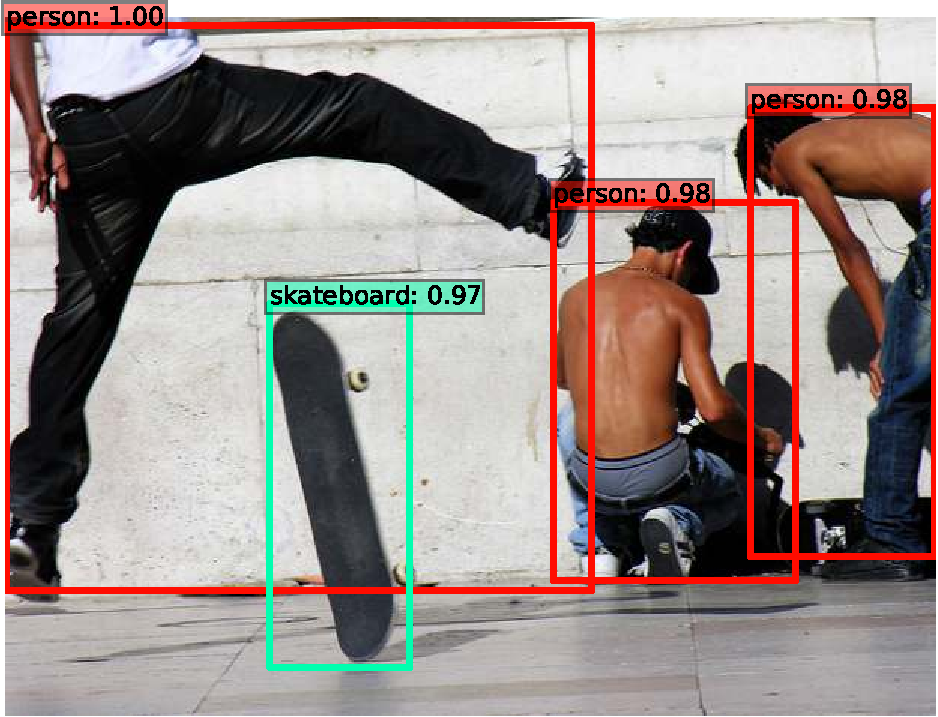
\includegraphics[width=0.22\linewidth]{ilustracije/coco/402750}
		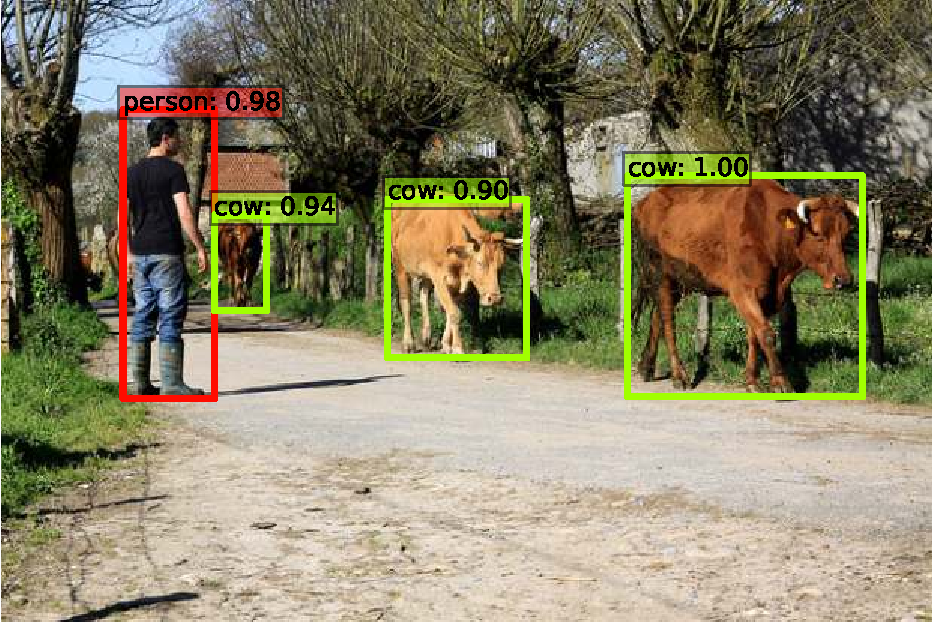
\includegraphics[width=0.22\linewidth]{ilustracije/coco/271809}
		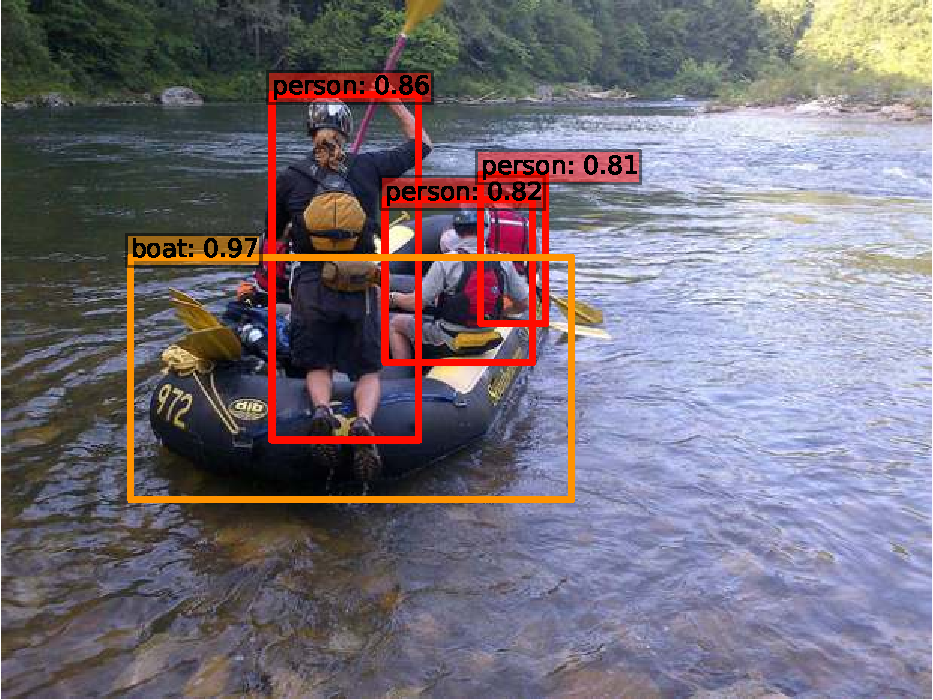
\includegraphics[width=0.22\linewidth]{ilustracije/coco/442079}\\
		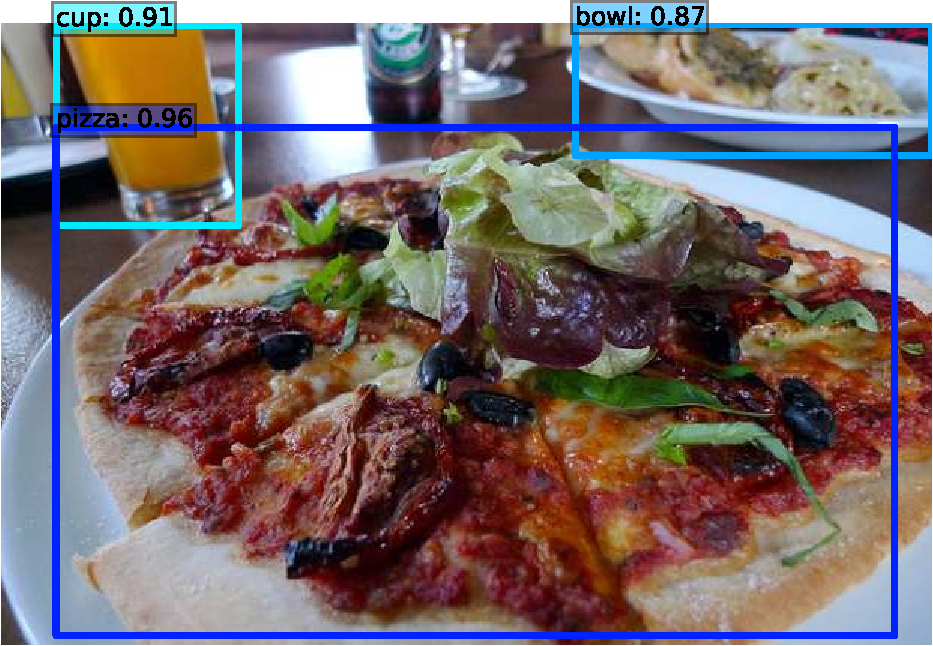
\includegraphics[width=0.22\linewidth]{ilustracije/coco/39662}
		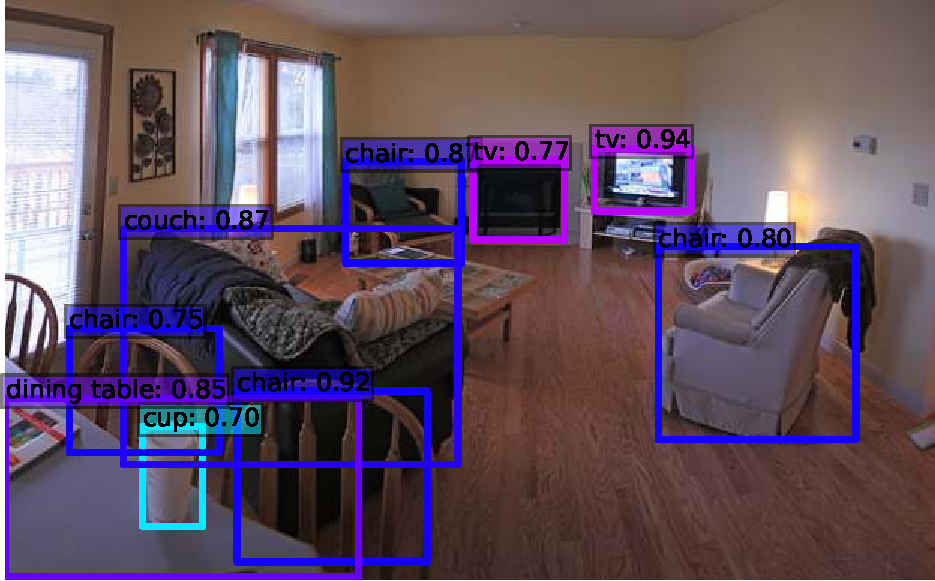
\includegraphics[width=0.22\linewidth]{ilustracije/coco/153988}
		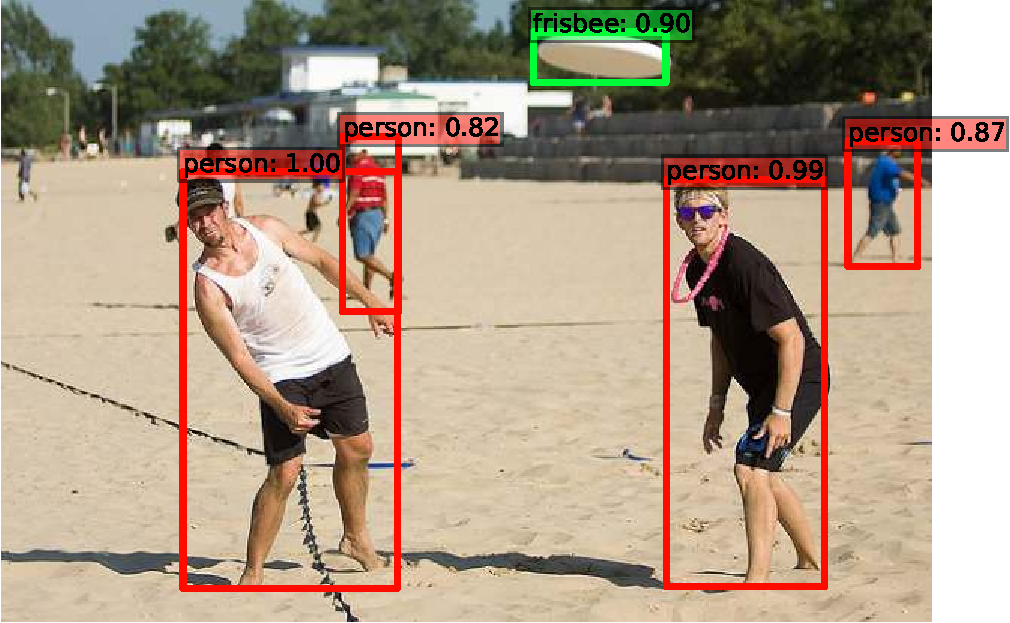
\includegraphics[width=0.22\linewidth]{ilustracije/coco/35114}
		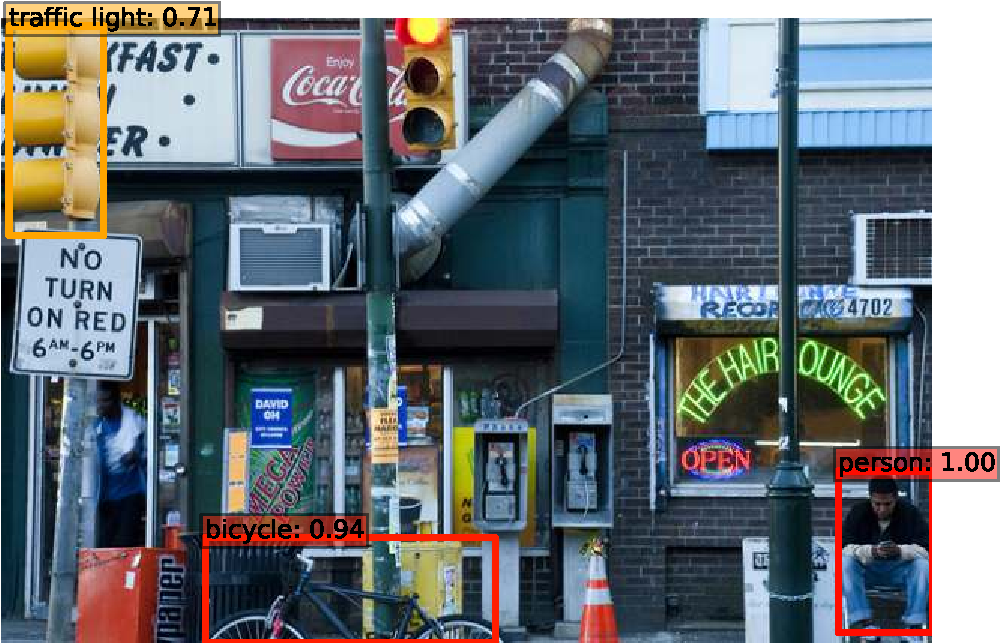
\includegraphics[width=0.22\linewidth]{ilustracije/coco/44974}\\
		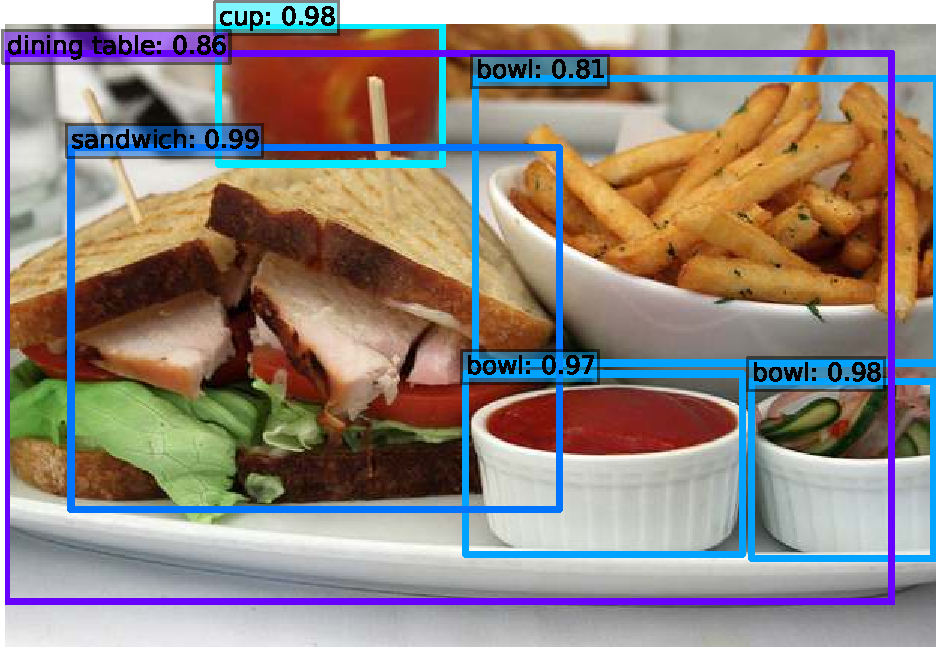
\includegraphics[width=0.22\linewidth]{ilustracije/coco/25090}
		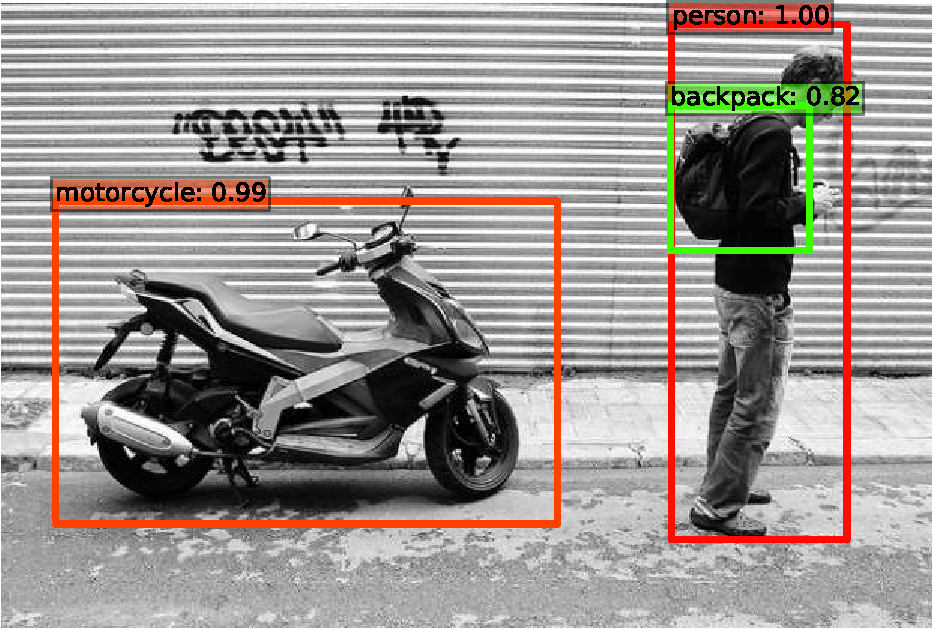
\includegraphics[width=0.22\linewidth]{ilustracije/coco/97838}
		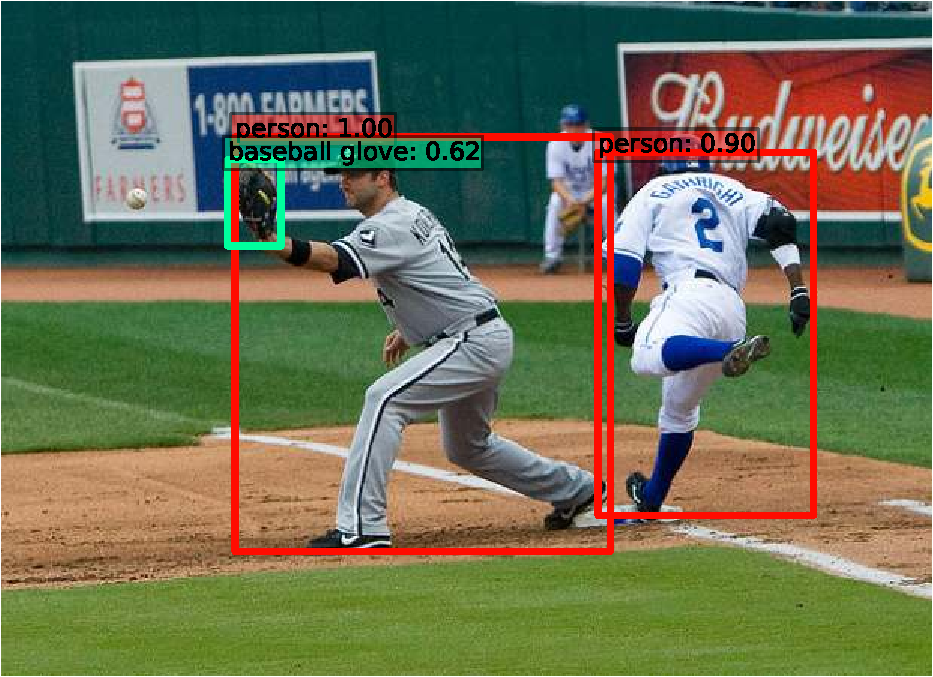
\includegraphics[trim={0 1.0cm 0 0},clip,width=0.22\linewidth]{ilustracije/coco/116280}
		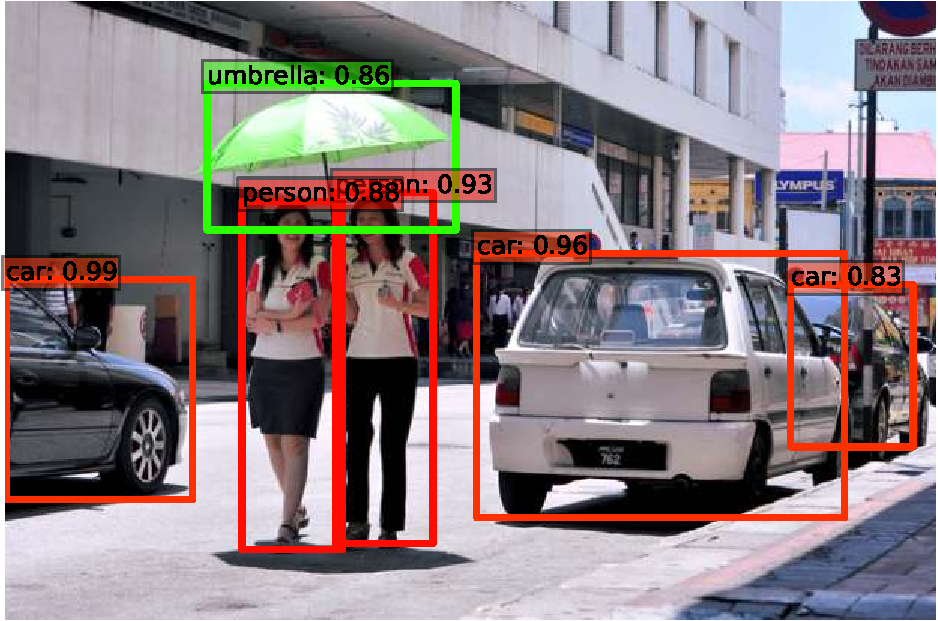
\includegraphics[width=0.22\linewidth]{ilustracije/coco/567767}\\
	%	}
		\caption{Primjeri rezultata pronalaženja objekata.}
		\label{fig:primjeri-rezultata-detekcije}
	\end{figure}
\end{frame}

\begin{frame}{Rezultati}
	\begin{figure}
		\centering
		%\resizebox{0.8\textwidth}{!}{%		
		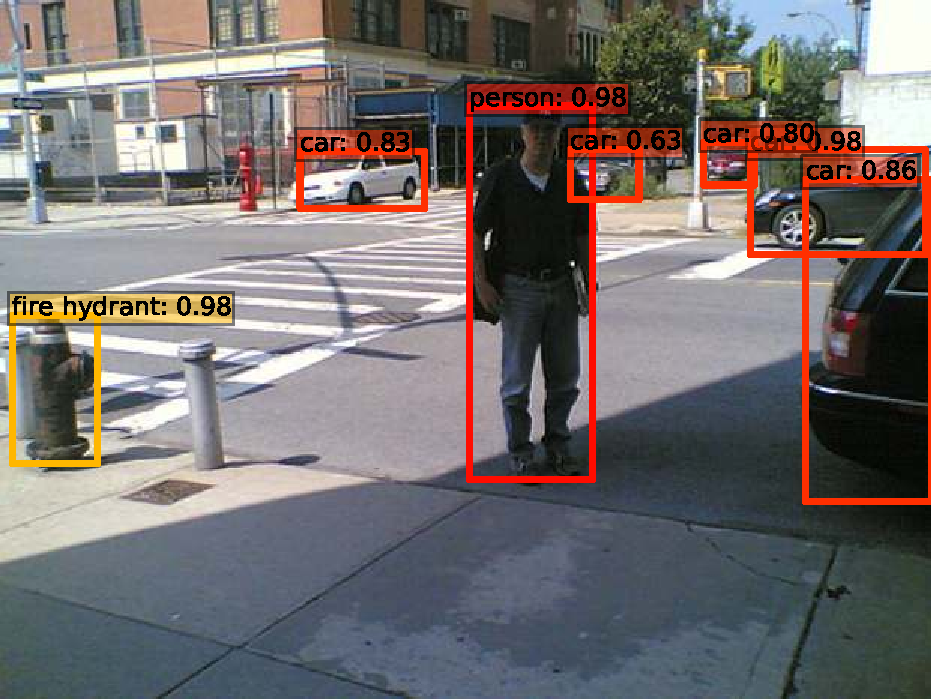
\includegraphics[width=0.22\linewidth]{ilustracije/coco/531694}
		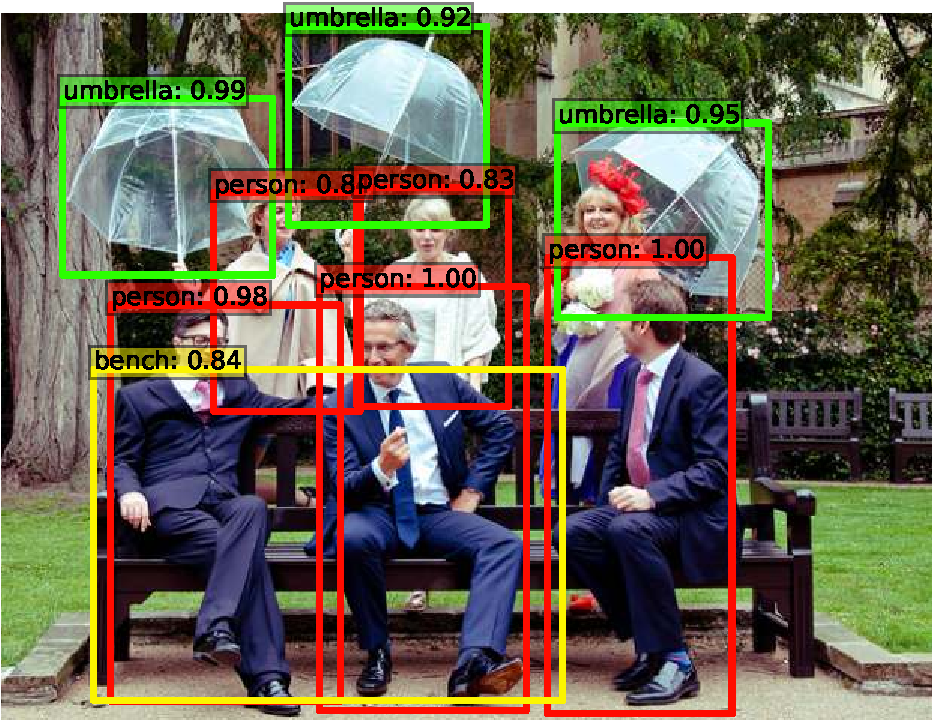
\includegraphics[width=0.22\linewidth]{ilustracije/coco/371251}
		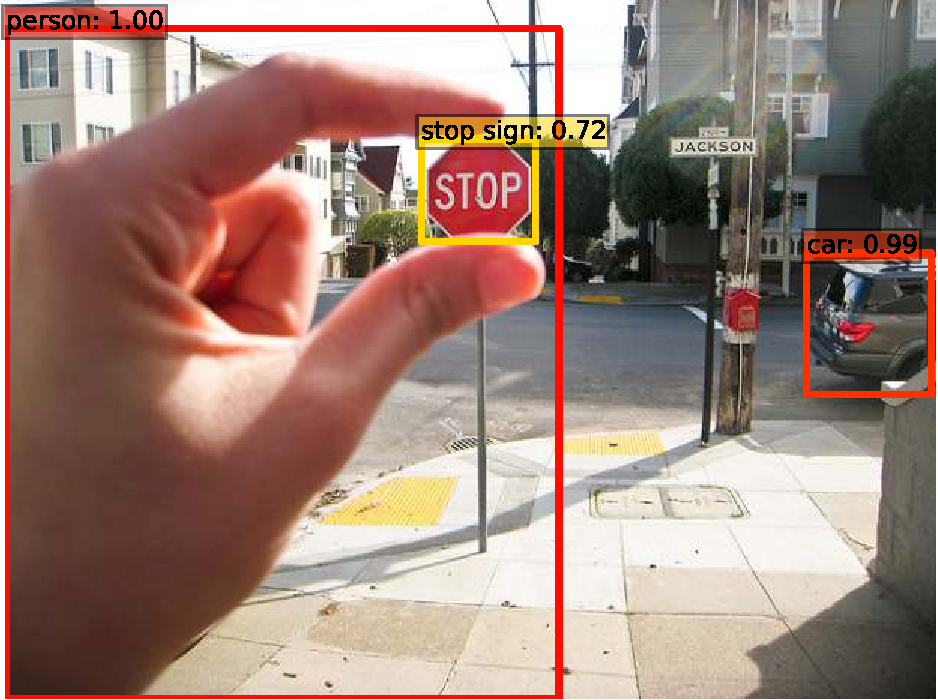
\includegraphics[width=0.22\linewidth]{ilustracije/coco/569617}
		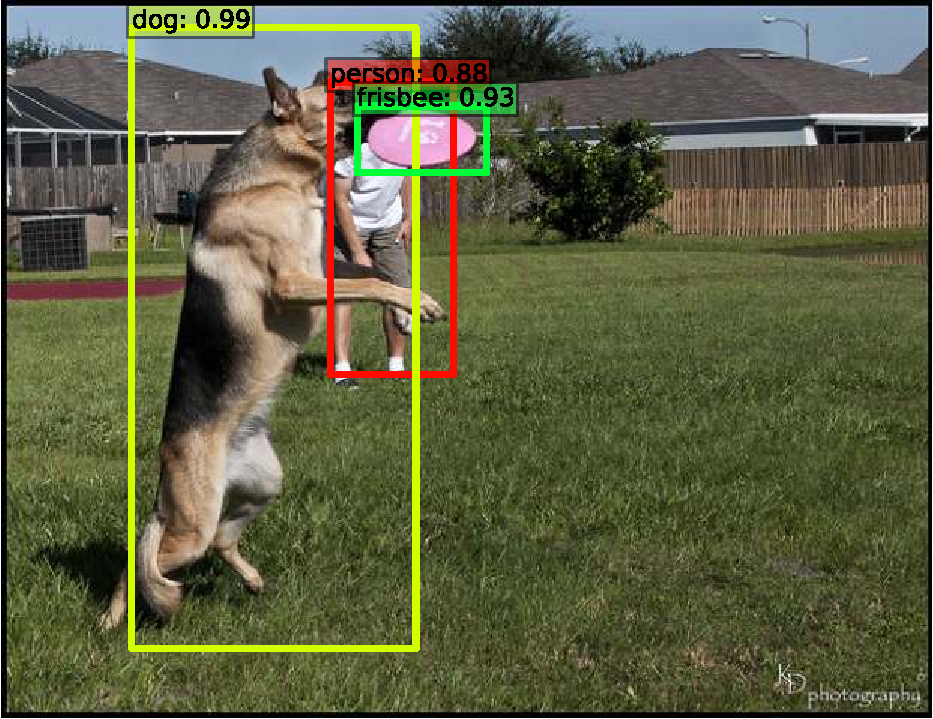
\includegraphics[width=0.22\linewidth]{ilustracije/coco/222239}\\
		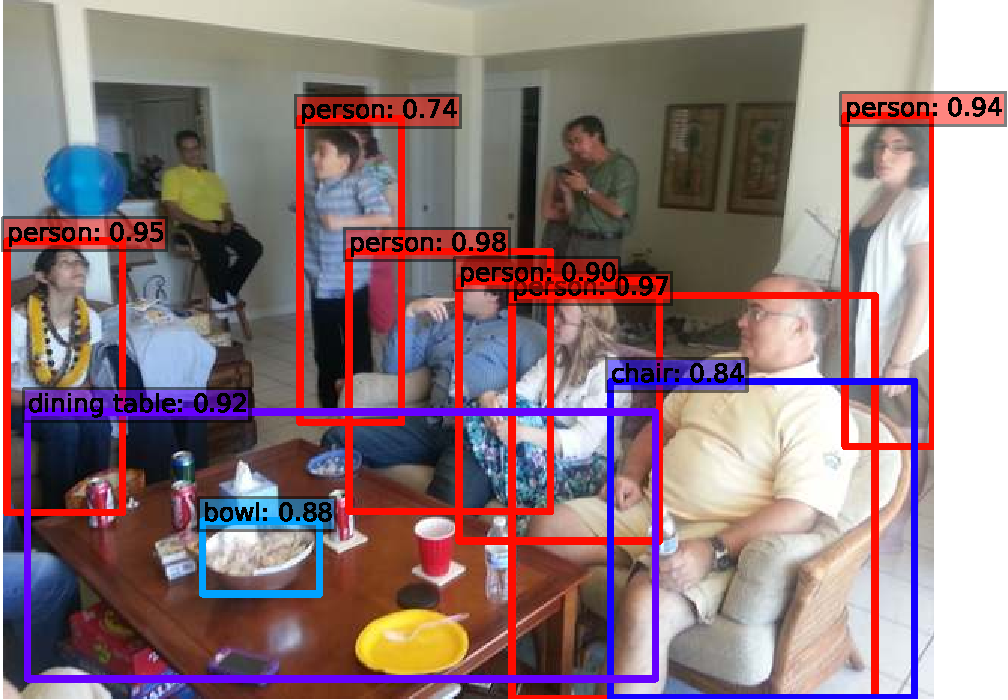
\includegraphics[trim={0 0 0 0.4cm},clip,width=0.22\linewidth]{ilustracije/coco/474449}
		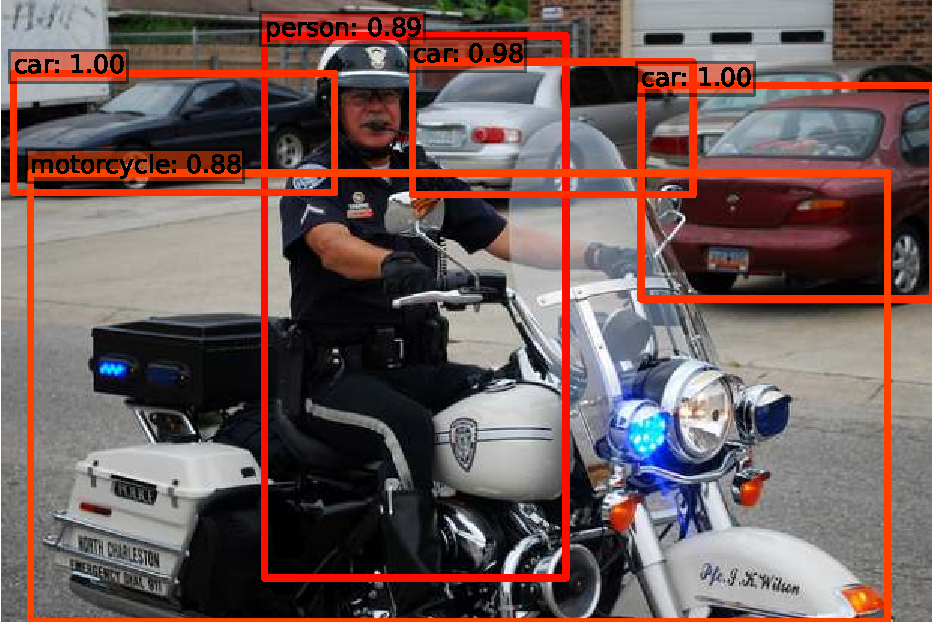
\includegraphics[width=0.22\linewidth]{ilustracije/coco/145416}
		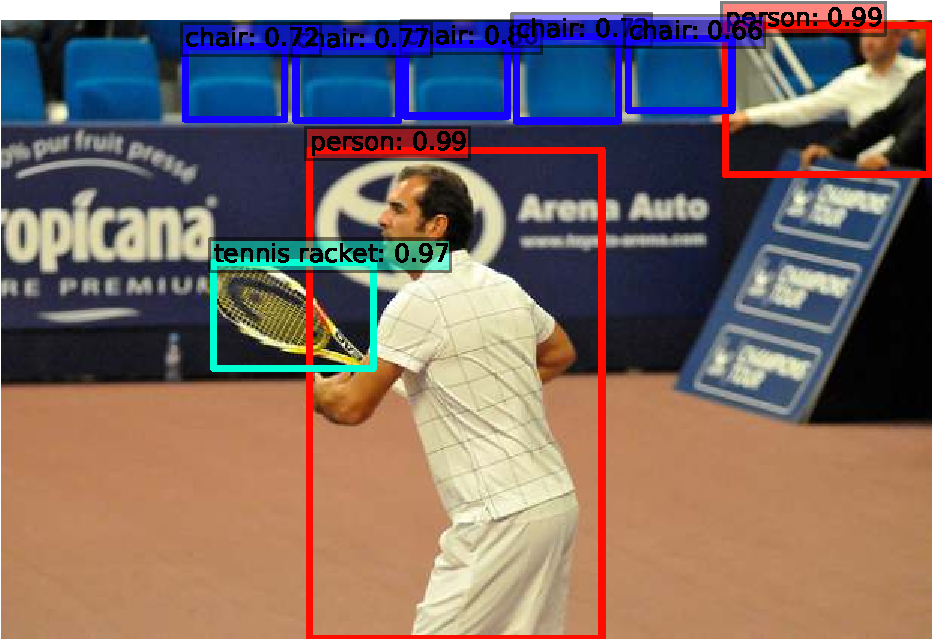
\includegraphics[width=0.22\linewidth]{ilustracije/coco/237488}
		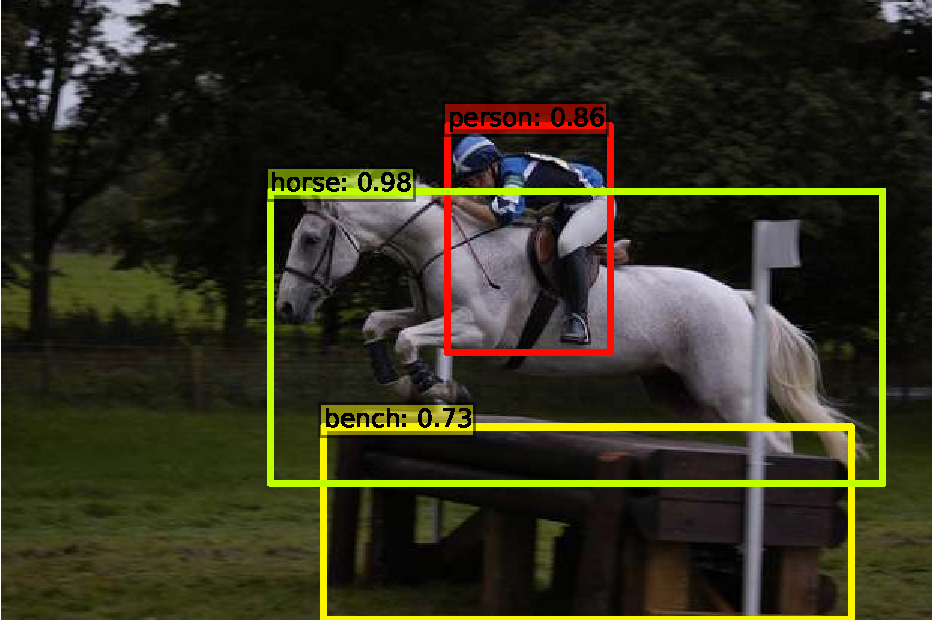
\includegraphics[width=0.22\linewidth]{ilustracije/coco/147107}\\
		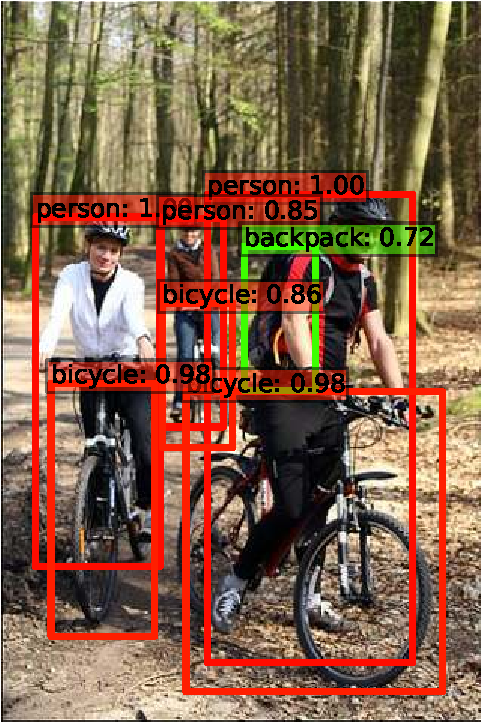
\includegraphics[trim={0 0 0 1.7cm},clip,width=0.22\linewidth]{ilustracije/coco/461193}
		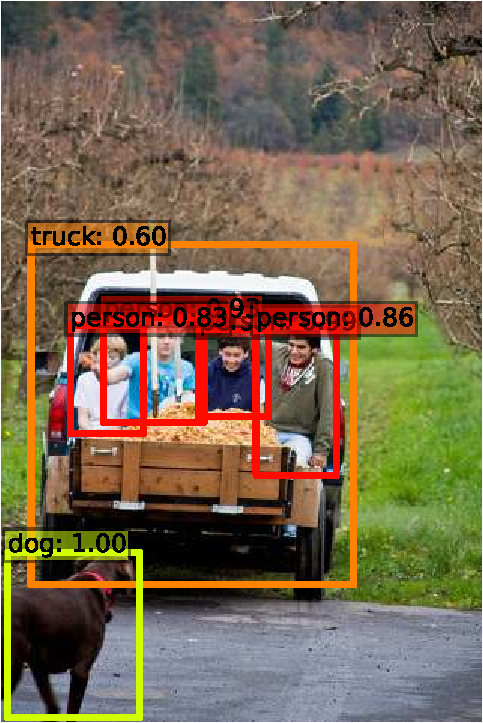
\includegraphics[trim={0 0 0 1.7cm},clip,width=0.22\linewidth]{ilustracije/coco/23408}
		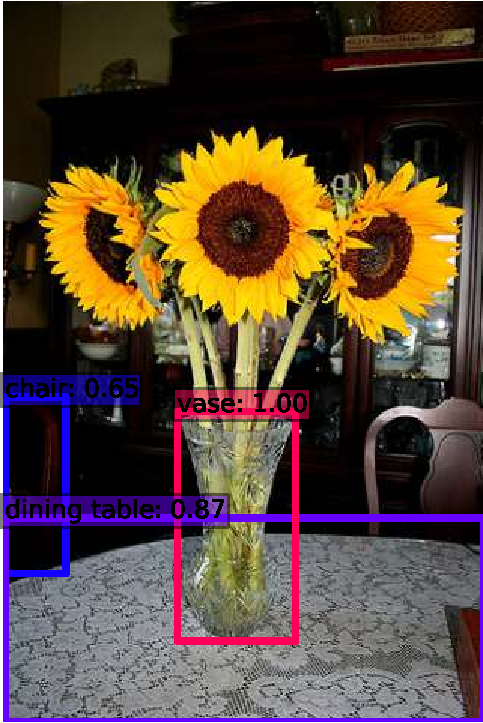
\includegraphics[trim={0 0 0 1.7cm},clip,width=0.22\linewidth]{ilustracije/coco/33705}
		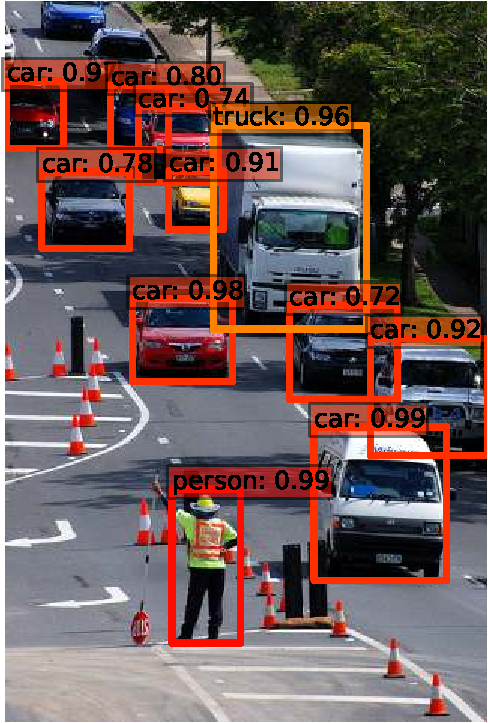
\includegraphics[trim={0 0 0 1.7cm},clip,width=0.22\linewidth]{ilustracije/coco/61871}\\
		%}
		\caption{Primjeri rezultata pronalaženja objekata.}
		\label{fig:primjeri-rezultata-detekcije}
	\end{figure}
\end{frame}

\end{document}
